% =====================================================================================
\section{Results: steering}
\label{sec:steering}
% =====================================================================================

The four structures are compared using three measures: the steering range at $S\ge0.8$, the power per degree, and
the settling time.

\subsection{Thermal kernels}
\label{sec:kernels}

\Cref{fig:kernels}(a) shows the temperature produced by one centred heater. On the \stack{standard} stack the heat
sink is \qty{2}{\micro\metre} below the cores. The core under the heater rises by \qty{0.196}{\KmW}
($\Ppi=\qty{19.7}{\milli\watt}$), and the profile has a half-width of \qty{3.3}{\micro\metre}: the cores 2, 4 and
\qty{8}{\micro\metre} away receive \num{0.75}, \num{0.41} and \num{0.12} of the peak, so $\Lth/d\approx1.7$. On the
\stack{undercut} membrane, heat can leave only sideways to the cavity walls and weakly through the air below. The
same heater raises its core by \qty{2.85}{\KmW} ($\Ppi=\qty{1.35}{\milli\watt}$), and the half-width is
\qty{20.6}{\micro\metre}: the cores 8, 16 and \qty{32}{\micro\metre} away receive \num{0.81}, \num{0.61} and \num{0.23}
of the peak, so $\Lth/d\approx10$ and one heater reaches the whole array. Both single-heater values agree with
measured devices of each kind (\cref{sec:fidelity}).

\begin{figure}[htbp]
  \centering
  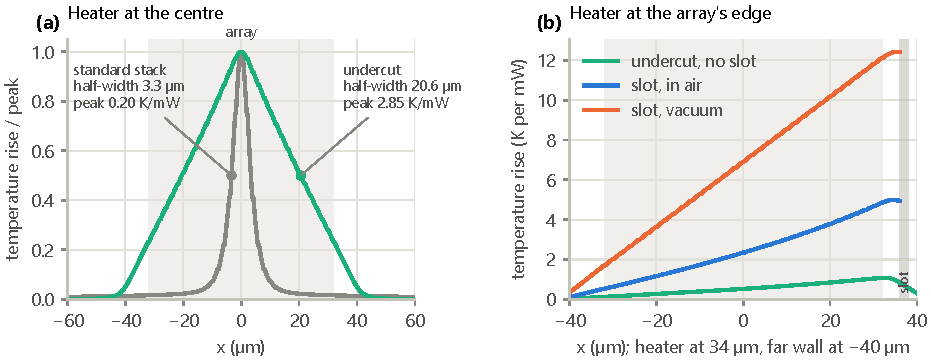
\includegraphics[width=\linewidth]{fig02_kernels}
  \caption{Temperature profile of one \qty{1}{\milli\metre} heater. (a)~Heater at the centre: half-width
  \qty{3.3}{\micro\metre} on the \stack{standard} stack and \qty{20.6}{\micro\metre} on the \stack{undercut}, which
  is \num{14} times hotter per milliwatt. (b)~Heater at the edge (\qty{34}{\micro\metre}): without a slot, little
  heat reaches the array; with a slot in air the profile is nearly linear; in vacuum it is linear and \num{2.5} times
  steeper.}
  \label{fig:kernels}
\end{figure}

\subsection{Standard stack}
\label{sec:standardfails}

On the \stack{standard} stack few heaters cannot steer. The best layout of eight heaters reaches a total span of
only \ang{3.4}, at \qty{60}{\mWdeg}: eight profiles \qty{3.3}{\micro\metre} wide leave most of the
\qty{64}{\micro\metre} aperture unheated. Steering one way across the full field requires \num{24} heaters. The
heated-section pitch matters as expected: \num{16} evenly spaced heaters steer \ang{18.6} at a
pitch of \qty{1.5}{\micro\metre} ($\Lth/d=2.2$) but only \ang{1.5} at \qty{4}{\micro\metre} ($\Lth/d=0.84$). With a
heater on every emitter and wrapped phases, the \stack{standard} stack needs \qtyrange{468}{580}{\milli\watt} between
\ang{1} and \ang{10}.
\subsection{Undercut membrane}
\label{sec:undercut}

On the \stack{undercut} membrane one edge heater already steers \ang{4.4}. Three heaters steer \ang{\pm 12} and four
reach \ang{\pm 16.0} at \qty{4.94}{\mWdeg}. With the outer pair placed just beyond the last emitters, four heaters
at $-32.75$, $-6.7$, $9.4$ and \qty{32.6}{\micro\metre} steer the full \ang{\pm 22.8} at \qty{5.24}{\mWdeg}.

The undercut design is inefficient. At \ang{10} it needs \qty{49}{\milli\watt}, while an ideal array of isolated
heaters with the same membrane's $\Ppi$ needs \qty{40}{\milli\watt}; the membrane is better only below about
\ang{8}. The reason is visible in \cref{fig:kernels}(b). An edge heater is \qty{8}{\micro\metre} from one cavity wall
and \qty{72}{\micro\metre} from the other. Each side conducts $\kt\,T_\mathrm{h}/\ell$ for a heater temperature $T_\mathrm{h}$, so the heat divides in inverse
proportion to the distances, and about \qty{90}{\percent} flows into the near wall without contributing to the ramp.

\subsection{Slot and vacuum}
\label{sec:slot}

If the membrane is cut just beyond the edge heater, the near wall can no longer be reached. All the heat must then
cross the array to the far wall, and with no losses in between the temperature is a straight line
(\cref{sec:superposition}).

\paragraph{Conduction limit.} The required power follows directly. All the heater power per unit length crosses the
membrane, $P/\Lh=\kt\,\dd T/\dd x$, and the steering angle sets the phase gradient,
$\Delta\phi/d=\gamma\Lh\,\dd T/\dd x$. Eliminating the gradient,
\begin{equation}
  P \;=\; \frac{\kt\,\Delta\phi}{\gamma\,d} \;=\; \qty{0.506}{\milli\watt}\ \text{per degree}
  \qquad(\kt=\qty{5.82e-6}{\watt\per\kelvin}).
  \label{eq:limit}
\end{equation}
This is independent of the number of emitters and of the heater length, because the same heat flux passes every
emitter. What grows with array size is the temperature at the hot end, proportional to $N$, and the settling time,
proportional to the square of the span.

\paragraph{Vacuum.} With no gas in the cavity or slot, one heater at \qty{34}{\micro\metre} produces a ramp straight
to \qty{0.016}{\percent} rms and steers the full \ang{22.8} at \qty{0.532}{\mWdeg} (\qty{5.3}{\milli\watt} at
\ang{10}), within \qty{5}{\percent} of \cref{eq:limit} with nothing fitted. Most of the difference is due to the
silicon cores, which add to the membrane's $\kt$, and the small residual gas conductivity. Additional heaters do not
reduce the power.

\paragraph{Air.} In air the single heater steers only \ang{4.0}, at \qty{1.30}{\mWdeg}. Two losses remain. Heat
escapes downward through the cavity air along the whole membrane, which curves the ramp (rms deviation
\qty{2.6}{\percent} of its rise, about \qty{1}{\rad} at \ang{10}). Air also conducts across the slot: its conductance
$k_\mathrm{air}t/w$ equals that of about \qty{106}{\micro\metre} of oxide membrane, comparable with the
\qty{74}{\micro\metre} path across the array.

Interior heaters correct the curvature (\cref{fig:placement}). With the edge heater at \qty{32}{\micro\metre}, a
second heater at \qty{5}{\micro\metre} extends the range to \ang{17.2}, and a third, with heaters at 2, 14 and
\qty{32}{\micro\metre}, reaches the full \ang{22.8} at
\begin{equation}
  \qty{1.38}{\mWdeg}, \quad\text{that is, } \qty{13.8}{\milli\watt}\ \text{at}\ \ang{10}.
\end{equation}
Of the \num{1891} three-heater layouts on a \qty{1}{\micro\metre} grid, \num{263} reach the full range, so the design
is not sensitive to exact positions. A \qty{4}{\micro\metre} slot reaching the wall reduces the power by a further
\qty{12}{\percent}, to \qty{1.22}{\mWdeg}.

\begin{figure}[htbp]
  \centering
  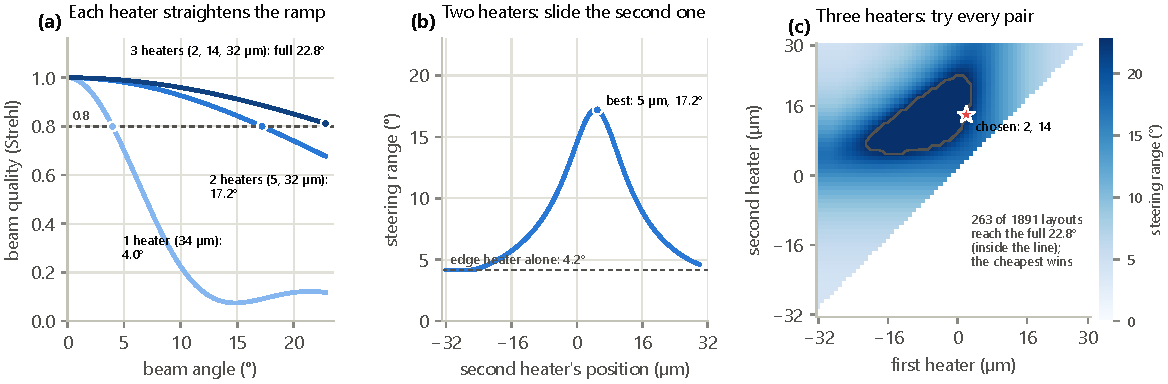
\includegraphics[width=\linewidth]{fig16_placement}
  \caption{Heater placement on the slot membrane. (a)~Strehl ratio against angle for the best layout of one, two and
  three heaters: ranges \ang{4.0}, \ang{17.2} and \ang{22.8}. (b)~Two heaters: range against the position of the
  second, edge heater at \qty{32}{\micro\metre}. (c)~Three heaters: range for every pair of interior positions;
  outlined layouts reach the full range.}
  \label{fig:placement}
\end{figure}

\Cref{fig:ramp} shows this design. The edge heater carries \qty{83}{\percent} of the power and produces the ramp;
the two interior heaters correct the curvature caused by the air loss. The resulting profile follows the ideal ramp
with $S=0.96$ at \ang{10}. Other angles require only scaling the three powers by $\sin\theta/\sin\ang{10}$.

\begin{figure}[htbp]
  \centering
  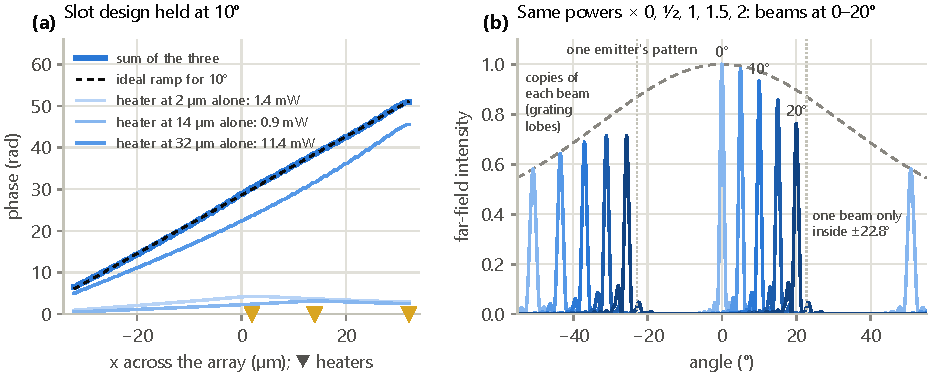
\includegraphics[width=\linewidth]{fig03_ramp_and_beams}
  \caption{The slot design (heaters at 2, 14 and \qty{32}{\micro\metre}). (a)~Phase at \ang{10}: each heater's
  contribution, their sum, and the ideal ramp. (b)~Far field at \ang{0}--\ang{20} in \ang{5} steps, powers scaled by
  $\sin\theta/\sin\ang{10}$. The dashed curve is the element pattern; each beam has a grating lobe at
  $\sin\theta-\lambda/d$.}
  \label{fig:ramp}
\end{figure}

\begin{table}[htbp]
  \centering
  \caption{Summary of the designs (simulated; $N=33$, $d=\qty{2}{\micro\metre}$). Range at $S\ge0.8$; ``$\pm$''
  denotes two-sided, otherwise one way. Settling is for a step from \ang{0} to \ang{10}.}
  \label{tab:designs}
  \footnotesize
  \setlength{\tabcolsep}{4.5pt}
  \begin{tabular}{@{}lcllccc@{}}
    \toprule
    Design & Wires & Heaters (\unit{\micro\metre}) & Range & \unit{\mWdeg} & $P_{10^\circ}$ (\unit{\milli\watt}) &
    Settling (\unit{\milli\second}) \\
    \midrule
    \stack{Standard}, isolated, wrapped & 33 & every emitter & \ang{\pm 22.8} & --- & 580 & $\approx0.02$\textsuperscript{a} \\
    \stack{Undercut} & 3 & $-8$, 10, 32 & \ang{15.9} & 4.93 & 49 & 2.0 \\
    \stack{Undercut}, heaters to the walls & 4 & $\pm32.7$, $-6.7$, 9.4 & \ang{\pm 22.8} & 5.24 & 52 & --- \\
    \stack{Slot} (air) & 3 & 2, 14, 32 & \ang{22.8} & 1.38 & 13.8 & 3.5 \\
    \stack{Vacuum} & 1 & 34 & \ang{22.8} & 0.53 & 5.3 & 8.8 \\
    \bottomrule
  \end{tabular}

  \vspace{2pt}
  \begin{minipage}{0.96\linewidth}\footnotesize
  \textsuperscript{a}\,Estimated from one heater's step response reaching \qty{92}{\percent}. Settling times of the
  membranes were computed for the nearest layouts on the \qty{4}{\micro\metre} grid of the transient runs
  (\stack{undercut} $-12$, 8, 32; \stack{slot} 0, 12, \qty{32}{\micro\metre}), whose powers differ by under
  \qty{1}{\percent}.
  \end{minipage}
\end{table}

\subsection{Comparison with a conventional array}
\label{sec:power}

\Cref{fig:power} compares the hold power with that of ideal conventional arrays. A wrapped array holds any angle
above about \ang{1.4} for roughly $0.9\,N\,\Ppi$, since no element needs more than $2\pi$. Our power grows with
$\sin\theta$, since the ramp is built in full. Per radian of phase the membrane is the more efficient actuator: the
\stack{vacuum} design uses \qty{7}{\micro\watt} per radian per emitter and the \stack{slot} design
\qty{18}{\micro\watt}, against \qty{16}{\micro\watt} for the best published folded phase shifter~\cite{lu2015} and
\qty{156}{\micro\watt} for the best single-pass suspended one~\cite{fang2011}. At \ang{10}, however, our ramp sums to
\qty{743}{\rad} over the array, while a wrapped array needs about \qty{92}{\rad}. As a result:
\begin{itemize}
  \item against a conventional \stack{standard}-stack array, the \stack{slot} and \stack{vacuum} designs need
        \num{42} and \num{110} times less power at \ang{10};
  \item against \num{33} single-pass suspended heaters (\qty{0.49}{\milli\watt}~\cite{fang2011}), the \stack{slot}
        design is lower below \ang{10.3} and equal at \ang{10};
  \item against \num{33} folded record shifters (\qty{50}{\micro\watt}~\cite{lu2015}), the \stack{vacuum} design is
        lower only below \ang{2.8} and \num{3.6} times higher at \ang{10}.
\end{itemize}
The last two cases are estimates for arrays that have not been built; they assume no crosstalk or calibration
power, and the record device is a \qty{6}{\milli\metre} folded Michelson switch.

\begin{figure}[htbp]
  \centering
  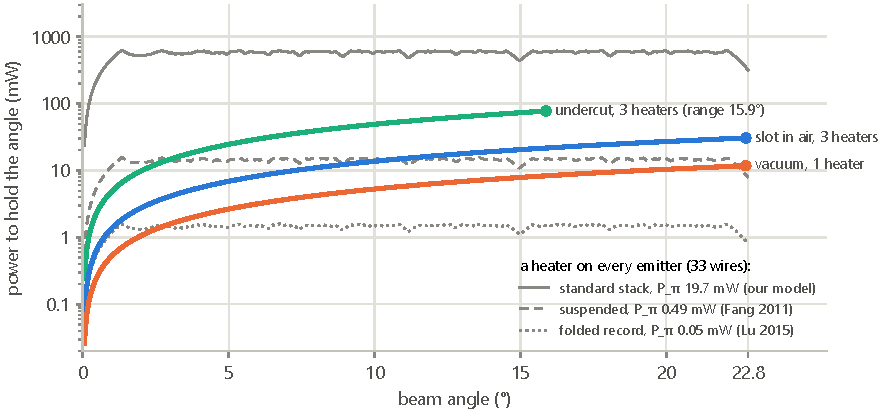
\includegraphics[width=0.86\linewidth]{fig04_power_vs_angle}
  \caption{Power to hold each angle, $N=33$. Grey: ideal conventional arrays (one isolated heater per emitter,
  wrapped phases) at three phase-shifter efficiencies. Colours: this work, one to three wires.}
  \label{fig:power}
\end{figure}

The slot and vacuum reduce power but not temperature. At \ang{10} the hottest core is \qtyrange{62}{64}{\kelvin}
above ambient for \qty{1}{\milli\metre} heaters in every design, because the required phase fixes it
($\Delta T=\phi/(\gamma\Lh)$); only a longer heater lowers it. A wrapped array never exceeds \qty{7.7}{\kelvin}.

\subsection{Speed}
\label{sec:speed}

A heater on the \stack{standard} stack warms its core to \qty{90}{\percent} in \qty{21}{\micro\second}; on the
\stack{undercut} membrane this takes \qty{1.63}{\milli\second}, \num{77} times longer for \num{14.5} times less power
(\cref{fig:transients}a). For a beam step from \ang{0} to \ang{10}, the Strehl ratio reaches and holds \num{0.8} after
\qty{2.0}{} (\stack{undercut}), \qty{3.5}{} (\stack{slot}) and \qty{8.8}{\milli\second} (\stack{vacuum}), that is,
bandwidths of roughly \num{190}, \num{110} and \qty{50}{\hertz} (\cref{fig:transients}b).

Two effects make these times long. First, a profile of spatial period $\Lambda$ relaxes at a rate
$\alpha(2\pi/\Lambda)^2+h/(\rho c\,t)$, so the ramp, the broadest profile, is the slowest; removing heat paths to save
power also removes paths by which the membrane settles, which is why vacuum is slower than air. Second, an
unwrapped \ang{10} ramp spans \qty{45}{\rad}, so the membrane must reach about \qty{99}{\percent} of its final state to
leave less than \qty{0.47}{\rad} of error, whereas a wrapped element needs about \qty{92}{\percent}. Small steps are
faster: a \ang{1} correction settles in \qty{0.36}{}, \qty{0.80}{} and \qty{2.4}{\milli\second}.

\begin{figure}[htbp]
  \centering
  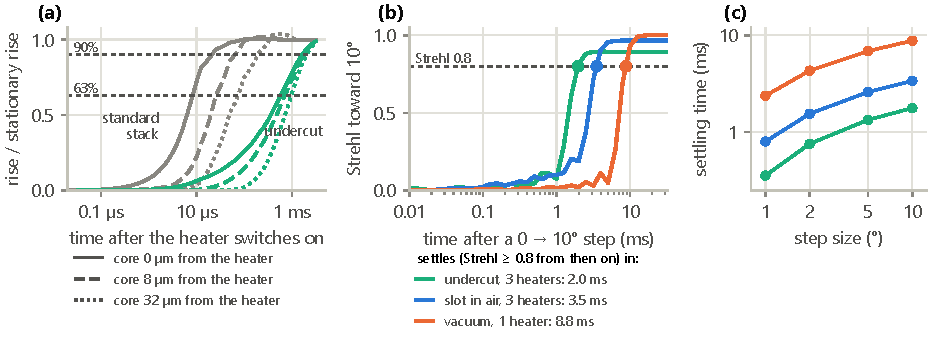
\includegraphics[width=\linewidth]{rep_transients}
  \caption{Speed with step drives. (a)~Single-heater step responses, \stack{standard} and \stack{undercut}.
  (b)~Strehl ratio towards \ang{10} after a step from \ang{0}. (c)~Settling time against step size.}
  \label{fig:transients}
\end{figure}

\subsection{Shaped drives (pre-emphasis)}
\label{sec:preemphasis}

A step drive is slow because each heater supplies only its final power from the start. Because conduction is
linear (\cref{sec:superposition}), the phase produced by any drive $P_k(t)$ is a sum of time-shifted step responses,
so the drive can be designed to reach the target sooner: each heater is first driven above its final power and then
brought back, and heaters whose heat arrives too strongly at some emitters are briefly turned down.

\paragraph{Method.} Each heater's drive is piecewise constant (30 intervals before the target time $T$, 15 after),
non-negative, and must end on the step's final powers, so every drive holds the same beam. The chip's total power
may not exceed $m$ times its hold power at \ang{10}. From $T$ onwards the rms phase error is required to stay below
$\sigma^*=\sqrt{2(1-\sqrt{0.8})}=\qty{0.46}{\rad}$, which guarantees $S\ge0.8$ since
$|\langle\ee^{\ii\varepsilon}\rangle|\ge1-\sigma^2/2$. This rms limit is a convex constraint, imposed with cutting
planes, so for each $T$ the drive is a linear program; bisection on $T$ gives the shortest settling time, and among
the drives that achieve it the one closest to the hold drive is kept. Two checks fix the method. For a single
thermal mode the optimal overdrive settles in $\tau\ln[m/(m-1+\varepsilon)]$, which the program reproduces to
\qty{0.3}{\percent}. With $m=1$ and one heater it returns the plain step. Doubling the time grids leaves $T$
unchanged. The settling times in this subsection are evaluated on a finer time grid than in \cref{sec:speed}, which
shortens the plain-step times by \qty{2.5}{\percent}.

\paragraph{Results.} With the chip allowed three times its hold power for a moment, a step from \ang{0} to \ang{10}
settles in \qty{0.43}{\milli\second} instead of \qty{3.42}{\milli\second} for the \stack{slot} design (\num{8} times
faster), \qty{1.43}{} instead of \qty{8.54}{\milli\second} in \stack{vacuum} (\num{6} times) and \qty{0.16}{} instead of
\qty{1.94}{\milli\second} on the \stack{undercut} (\num{12} times) (\cref{fig:preemphasis}). At twice the hold power the
gains are \numrange{4}{9} times. The extra energy per step is \qtyrange{9}{13}{\micro\joule}.

The gain comes from driving the heaters independently. One overdrive waveform shared by all heaters gives only
\numrange{3}{4} times, and overheats the hottest core to \numrange{1.5}{2.3} times its final temperature; with
independent drives the hottest core stays within \qty{8}{\percent} of its final value for the \stack{slot} design.
Two heaters already give \num{7.3} times, and seventeen give \num{10.7} times, so the few-wire design keeps most of
the available gain. Small corrections gain most: a \ang{1} step from a held angle settles \numrange{10}{19} times
faster. A return to \ang{0} cannot be accelerated, since all heaters are then already off; if fast returns matter,
the rest position can be set at a small standing tilt.

\paragraph{Sensitivity.} The drive is computed from the thermal model, so it depends on the model's time scale. If
the device's heat flow is \qty{2}{\percent} slower than modelled, the \stack{slot} design's \num{8}-fold gain falls to
about \num{3}; the planned cut-back then arrives before the heat. A drive designed to work over a $\pm\qty{5}{\percent}$
range of time scales keeps a gain of \num{6.8} (\qty{0.51}{\milli\second}) for the \stack{slot} design and \num{5.6}
(\qty{1.54}{\milli\second}) in \stack{vacuum}, and \ang{1} corrections lose less than \qty{20}{\percent} of their gain for
a $\pm\qty{10}{\percent}$ error. In practice each heater's step response would be measured on the device before the
drives are computed.

\begin{figure}[htbp]
  \centering
  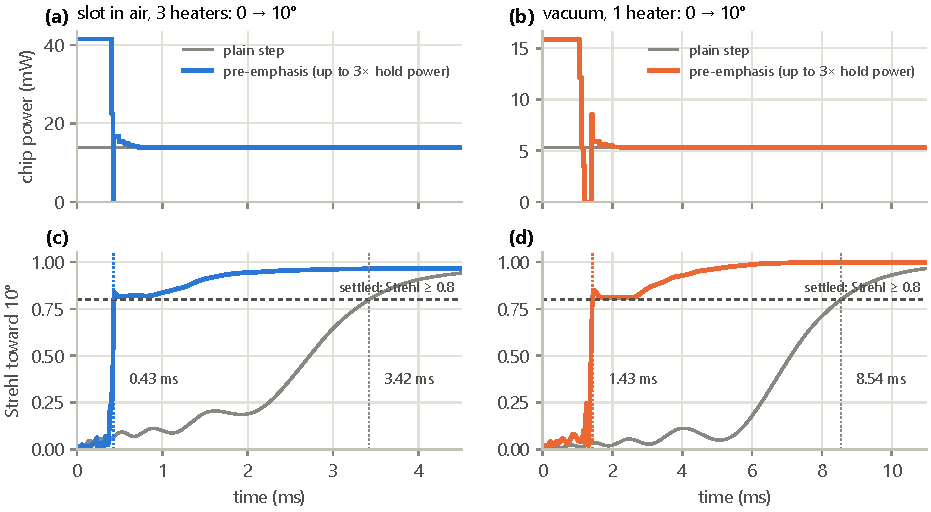
\includegraphics[width=\linewidth]{fig06_preemphasis}
  \caption{Pre-emphasis for a step from \ang{0} to \ang{10}. (a,~b)~Total chip power for the plain step and for the
  optimised drive, limited to three times the hold power, for the \stack{slot} (three heaters) and \stack{vacuum} (one
  heater) designs. (c,~d)~Strehl ratio towards \ang{10}; the settling time is where it last crosses \num{0.8}.}
  \label{fig:preemphasis}
\end{figure}

\Cref{fig:powerspeed} plots hold power against settling time. Along the design path each structure trades speed for
power. With plain steps, the product of power and settling time for a \ang{10} step is about
\qty{14}{\milli\watt\,\milli\second} for the conventional \stack{standard} array and
\qtyrange{46}{96}{\milli\watt\,\milli\second} for the membranes, against \numrange{0.5}{5} for published phase
shifters scaled to \num{33} elements. With pre-emphasis the membranes reach \qtyrange{6}{8}{\milli\watt\,\milli\second},
within \numrange{1.2}{16} times of the published devices driven with plain steps, and level with them for small
corrections.

\begin{figure}[htbp]
  \centering
  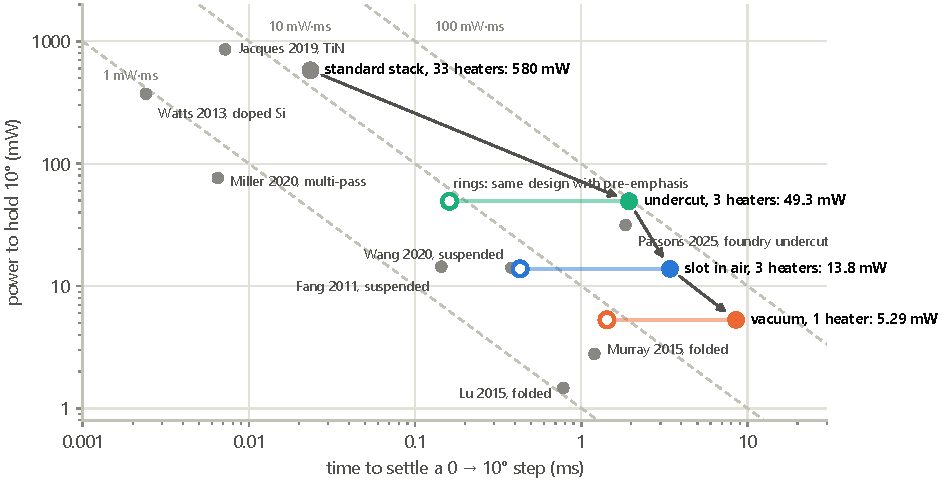
\includegraphics[width=0.9\linewidth]{fig05_power_vs_speed}
  \caption{Power to hold \ang{10} against the time to settle a step from \ang{0}. Filled circles: the four
  structures with a plain step. Rings: the same designs with pre-emphasis at up to three times the hold power. Grey:
  published single phase shifters~\cite{jacques2019,watts2013,miller2020,wang2020,fang2011,parsons2025,murray2015,lu2015}
  scaled to \num{33} isolated, wrapped heaters at their measured $\Ppi$, with the slower of their rise and fall
  times (our estimate). Dashed: constant power $\times$ time.}
  \label{fig:powerspeed}
\end{figure}
